\newpage

\chapter{Architettura del sistema e scelte progettuali}

In questo capitolo vengono descritte le scelte progettuali e l'architettura del sistema implementato, con particolare enfasi sul protocollo di comunicazione.

\section{Introduzione}
Lo scopo del progetto è progettare ed implementare un'applicazione client-server per il trasferimento di file in linguaggio C, utilizzando l'API dei socket di Berkeley.
L'applicazione dovrà impiegare il servizio di rete senza connessione, ossia il protocollo UDP (socket di tipo \lstinlinebg{SOCK_DGRAM}) per la trasmissione dei dati.
Il software deve permettere:
\begin{itemize}
    \item La connessione client-server senza autenticazione;
    \item La visualizzazione sul client dei file disponibili sul server tramite il comando \lstinlinebg{LIST};
    \item Il download di un file dal server tramite il comando \lstinlinebg{GET};
    \item L'upload di un file sul server tramite il comando \lstinlinebg{PUT};
    \item Il trasferimento di file in modo affidabile.
\end{itemize}
La comunicazione tra client e server deve avvenire tramite un opportuno protocollo.
Il protocollo di comunicazione deve prevedere lo scambio di due tipi di messaggi:
\begin{itemize}
    \item \textit{messaggi di comando}: vengono inviati dal client al server per richiedere delle diverse operazioni;
    \item \textit{messaggi di risposta}: vengono inviati dal server al client, in risposta ad un comando, con l'esito dell'operazione.
\end{itemize}

\subsection{Funzionalità del server \emoji{file-cabinet}}
Il server, di tipo concorrente, deve fornire le seguenti funzionalità:
\begin{itemize}
    \item L'invio del messaggio di risposta al comando \lstinlinebg{LIST} al client richiedente; il messaggio di risposta contiene la lista dei file, ovvero la lista dei nomi dei file disponibili per la condivisione;
    \item L'invio del messaggo di risposta al comando \lstinlinebg{GET} contenente il file richiesto, se presente, o un opportuno messaggio di errore;
    \item La ricezione di un messaggio \lstinlinebg{PUT} contenente il file da caricare sul server e l'invio di un messaggio di risposta con l'esito dell'operazione.
\end{itemize}

\subsection{Funzionalità del client \emoji{bust-in-silhouette}}
Il client, di tipo concorrente, deve fornire le seguenti funzionalità:
\begin{itemize}
    \item L'invio del messaggio \lstinlinebg{LIST} per richiedere la lista dei nomi dei file disponibili;
    \item L'invio del messaggio \lstinlinebg{GET} per ottenere un file;
    \item La ricezione di un file, richiesta tramite il messaggio di \lstinlinebg{GET}, o la gestione dell'eventuale errore;
    \item L'invio del messaggio \lstinlinebg{PUT} per effettuare l'upload di un file sul server e la ricezione del messaggio di risposta con l'esito dell'operazione.
\end{itemize}

\begin{figure}[h]
    \centering
    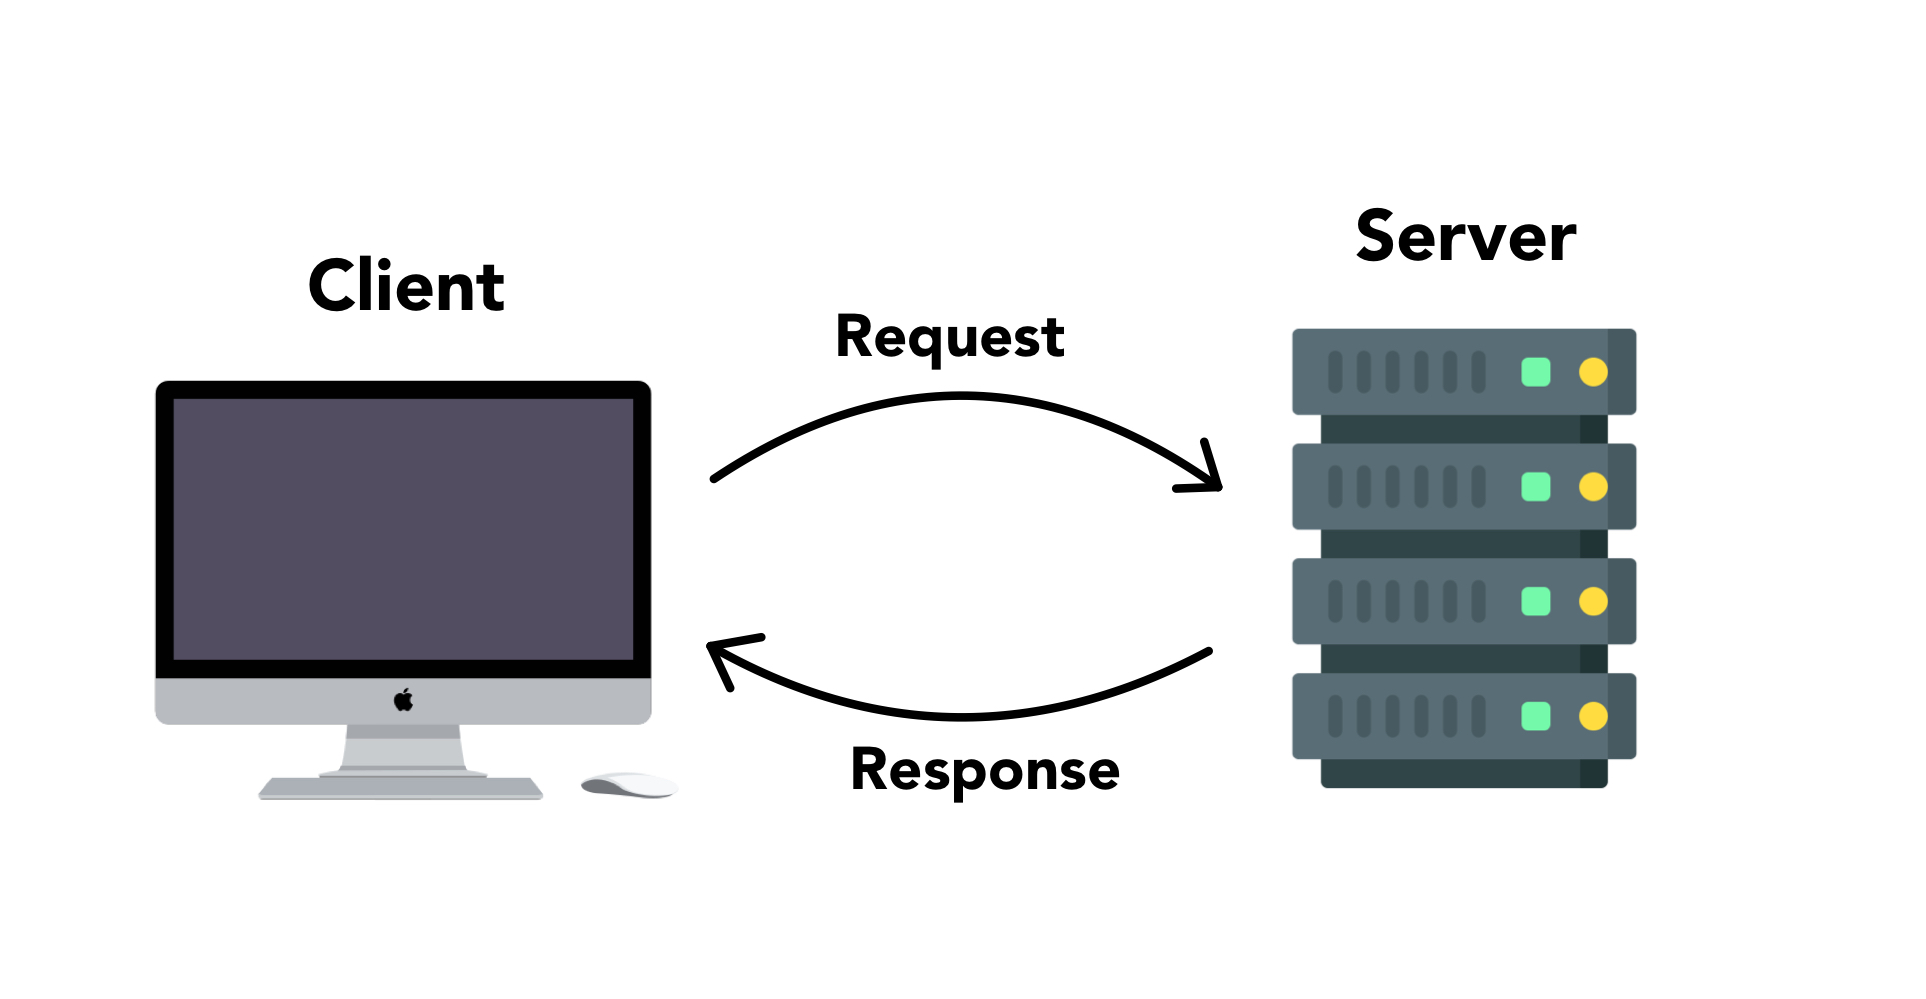
\includegraphics[width=0.6\textwidth]{imgs/01/client-server.jpeg}
    \caption{Schema client-server}
\end{figure}

\subsection{Trasmissione affidabile \emoji{handshake}}
Lo scambio di messaggi avviene usando un servizio di comunicazione non affidabile.
Al fine di garantire la corretta spedizione/ricezione dei messaggi e dei file sia i client che il server implementano a livello applicativo il protocollo \textit{Selective Repeat} con finestra di spedizione \lstinlinebg{WINDOW_SIZE}.
Per simulare la perdita dei messaggi in rete (evento alquanto improbabile in una rete locale per non parlare di quando client e server sono eseguiti sullo stesso host), si assume che ogni messaggio sia scartato dal mittente con probabilità \lstinlinebg{LOSS_PROBABILITY}.
La dimensione della finestra di spedizione \lstinlinebg{WINDOW_SIZE}, la probabilità di perdita dei messaggi \lstinlinebg{LOSS_PROBABILITY}, e la durata del timeout \lstinlinebg{TIMEOUT}, sono tre costanti configurabili ed uguali per tutti i processi.
Oltre all'uso di un timeout fisso (\textit{static timeout}), deve essere possibile scegliere l'uso di un valore per il timeout adattativo (\textit{adaptive timeout}) calcolato dinamicamente in base all'evoluzione dei ritardi di rete osservati.
I client ed il server devono essere eseguiti nello spazio utente senza richiedere privilegi di root.
Il server deve essere in ascolto su una porta di default (configurabile).

\section{Architettura del sistema \emoji{gear}}

\subsection{Organizzazione del progetto}
Il progetto S.P.Q.R. (\textit{Selective Protocol for Quality and Reliability}) consta di diverse directory\footnote{Si vuole specificare che la \textit{working directory} \lstinlinebg{spqr/} è composta fondamentalmente dalle directory citate.}, tra le più d'interesse troviamo:
\begin{itemize}
    \item \emoji{file-folder}\lstinlinebg{src/}: contiene i sorgenti del progetto, organizzato in file dedicati per lo sviluppo di specifiche funzionalità per il client e per il server;
    \item \emoji{file-folder}\lstinlinebg{include/}: contiene gli header del progetto, organizzati per modularità e riutilizzo del codice;
    \item \emoji{file-folder}\lstinlinebg{client-files/} e \emoji{file-folder}\lstinlinebg{server-files/}: nelle quali troviamo i file che il client e il server si scambiano tra loro;
    \item \emoji{file-folder}\lstinlinebg{tests/}: nella quale è presente lo script \lstinlinebg{integrity-consistency.py} che controlla l'integrità di ogni file inviato e/o ricevuto dal client e dal server;
    \item \emoji{file-folder}\lstinlinebg{tests/network/}: nella quale è presente lo script \lstinlinebg{list.pcapng} che riporta il traffico di rete generato dal client e dal server durante l'esecuzione del comando \lstinlinebg{LIST};
    \item \emoji{file-folder}\lstinlinebg{tests/performance/}: nella quale si trovano i grafici delle performance relativi al timeout statico, al timeout adattivo e alla comulazione degli errori;
    \item \emoji{file-folder} \lstinlinebg{docs/}: nella quale si trova il sito web del progetto.
\end{itemize}
Oltre alle directory citate, troviamo il \emoji{wrench}\lstinlinebg{Makefile} di particolare rilievo per automatizzare la compilazione del progetto.
Entrando più nel dettaglio, nella directory \lstinlinebg{src/} troviamo i seguenti file:
\begin{itemize}
    \item \emoji{page-facing-up}\lstinlinebg{client.c}: rappresenta il punto d'ingresso del client ed in particolare si occupa di gestire l'argomento \lstinlinebg{IPv4} (cioè l'indirizzo IP del server a cui i client devono connettersi) tramite riga di comando, istanzia il gestore dei segnali e tenta l'avvio della connesione con il server;
    \item \emoji{page-facing-up}\lstinlinebg{server.c}: rappreenta il punto d'ingresso del server, configura il socket principale, gestisce le connesioni in entrata e istanzia il gestore dei segnali;
    \item \emoji{page-facing-up}\lstinlinebg{common.c}: contiene funzioni e strutture condivise tra client e server (es: gestione timeout, progress bar, ASCII art, gestione degli errori, simulazione perdita pacchetti, ...);
    \item \emoji{page-facing-up}\lstinlinebg{protocol.c}: implementa il protocollo di trasferimento dati implementando il \textit{Selective Repeat} \emoji{incoming-envelope};
    \item \emoji{page-facing-up}\lstinlinebg{spqr_client.c}: implementa la logica del client, l'invio/ricezione pacchetti, comandi utente \lstinlinebg{LIST}, \lstinlinebg{GET}, \lstinlinebg{PUT} e gestione del comando aggiuntivo \lstinlinebg{CLOSE};
    \item \emoji{page-facing-up}\lstinlinebg{spqr_server.c}: implementa la logica del server, la gestione concorrente di client multipli e la bitmask per tracciare le connessioni attive.
\end{itemize}
Mentre, per quanto riguarda la directory \lstinlinebg{include/}, troviamo i seguenti file:
\begin{itemize}
    \item \emoji{page-facing-up}\lstinlinebg{stdc.h}: contiene tutte le librerie standard del linguaggio C e file header custom come \lstinlinebg{settings.h} e \lstinlinebg{common.h};
    \item \emoji{page-facing-up}\lstinlinebg{settings.h}: contiene le configurazioni globali e i parametri del progetto (es: il numero di porta, il numero massimo di client supportati, il timeout statico, il timeout adattivo, la dimensione della finestra, la probabilità di perdita, ...);
    \item \emoji{page-facing-up}\lstinlinebg{common.h}: contiene i prototipi delle funzioni e dei messaggi custom condivisi tra client e server;
    \item \emoji{page-facing-up}\lstinlinebg{protocol.h}: definizione delle strutture utili per il protocollo di trasferimento dati in modo affidabile implementanto tramite \textit{Selective Repeat} \emoji{incoming-envelope};
    \item \emoji{page-facing-up}\lstinlinebg{spqr_client.h}: prototipi della funzioni specifiche del client (es: gestione delle connesioni (\textit{Three-Way Handshake} con il server), gestione della terminazione con \lstinlinebg{ctrl+c}, ...);
    \item \emoji{page-facing-up}\lstinlinebg{spqr_server.h}: prototipi della funzioni specifiche del server (es: supporto a client multipli via \lstinlinebg{fork()}, risposta ai comandi \lstinlinebg{LIST}, \lstinlinebg{GET}, \lstinlinebg{PUT} e gestione del comando aggiuntivo \lstinlinebg{CLOSE}, ...).
\end{itemize}

\subsection{Protocollo Selective Repeat \emoji{incoming-envelope}}
L'architettura client-server progettata utilizza il protocollo di comunicazione non affidabile UDP per il trasferimento dei messaggi.
Tuttavia, per garantire l'affidabilità nella trasmissione dei file tra client e server, è stato implementato il protocollo \textit{Selective Repeat} \emoji{incoming-envelope}.
Questo protocollo ottimizza la gestione degli errori, riducendo al minimo le ritrasmissioni grazie alla selezione mirata dei pacchetti persi o corrotti, migliorando così l'efficienza complessiva del sistema.

\subsubsection{Funzionamento generale}
Il protocollo \textit{Selective Repeat} si basa sull'uso di una finestra scorrevole condivisa tra mittente e destinatario, consentendo l'invio e la ricezione di più pacchetti senza dover attendere una conferma immediata.
La dimensione della finestra determina il numero massimo di pacchetti che possono essere ``in volo" contemporaneamente.
Ogni pacchetto trasmesso è identificato da un numero di sequenza univoco, che permette al destinatario di riordinare correttamente i dati ricevuti.

A differenza di altri protocolli di affidabilità, il \textit{Selective Repeat} \emoji{incoming-envelope} utilizza ACK selettivi, ovvero conferme individuali per ogni pacchetto ricevuto, anche se fuori ordine.
I pacchetti non ancora riordinabili vengono temporaneamente memorizzati in un buffer, in attesa di ricevere quelli mancanti.

\subsubsection{Comportamento del Mittente}
Il mittente gestisce la trasmissione dei pacchetti rispettando la finestra di invio.
Ogni pacchetto viene inviato con un timer individuale che controlla il tempo massimo di attesa per la conferma.

Quando il mittente riceve un ACK, il pacchetto corrispondente viene marcato come confermato e la finestra scorre, consentendo l'invio di nuovi dati.
Se il timer di un pacchetto scade senza che sia stato ricevuto un ACK, il pacchetto viene ritrasmesso selettivamente, evitando di reinviare quelli già confermati.

\subsubsection{Comportamento del Destinatario}
Il destinatario, una volta ricevuti i pacchetti, segue una logica basata su bufferizzazione e riordinamento:
\begin{itemize}
    \item Accetta i pacchetti anche se ricevuti fuori ordine.
    \item I pacchetti non immediatamente utilizzabili vengono temporaneamente salvati in un buffer.
    \item Ogni pacchetto ricevuto genera un ACK, inviato al mittente indipendentemente dalla ricezione dei pacchetti precedenti.
    \item Se un pacchetto è già stato confermato in precedenza, eventuali ACK duplicati vengono ignorati dal mittente.
    \item Una volta ricevuti tutti i pacchetti fino a un certo numero di sequenza, i dati vengono consegnati all'applicazione in modo ordinato.
\end{itemize}

\begin{figure}[h]
    \centering
    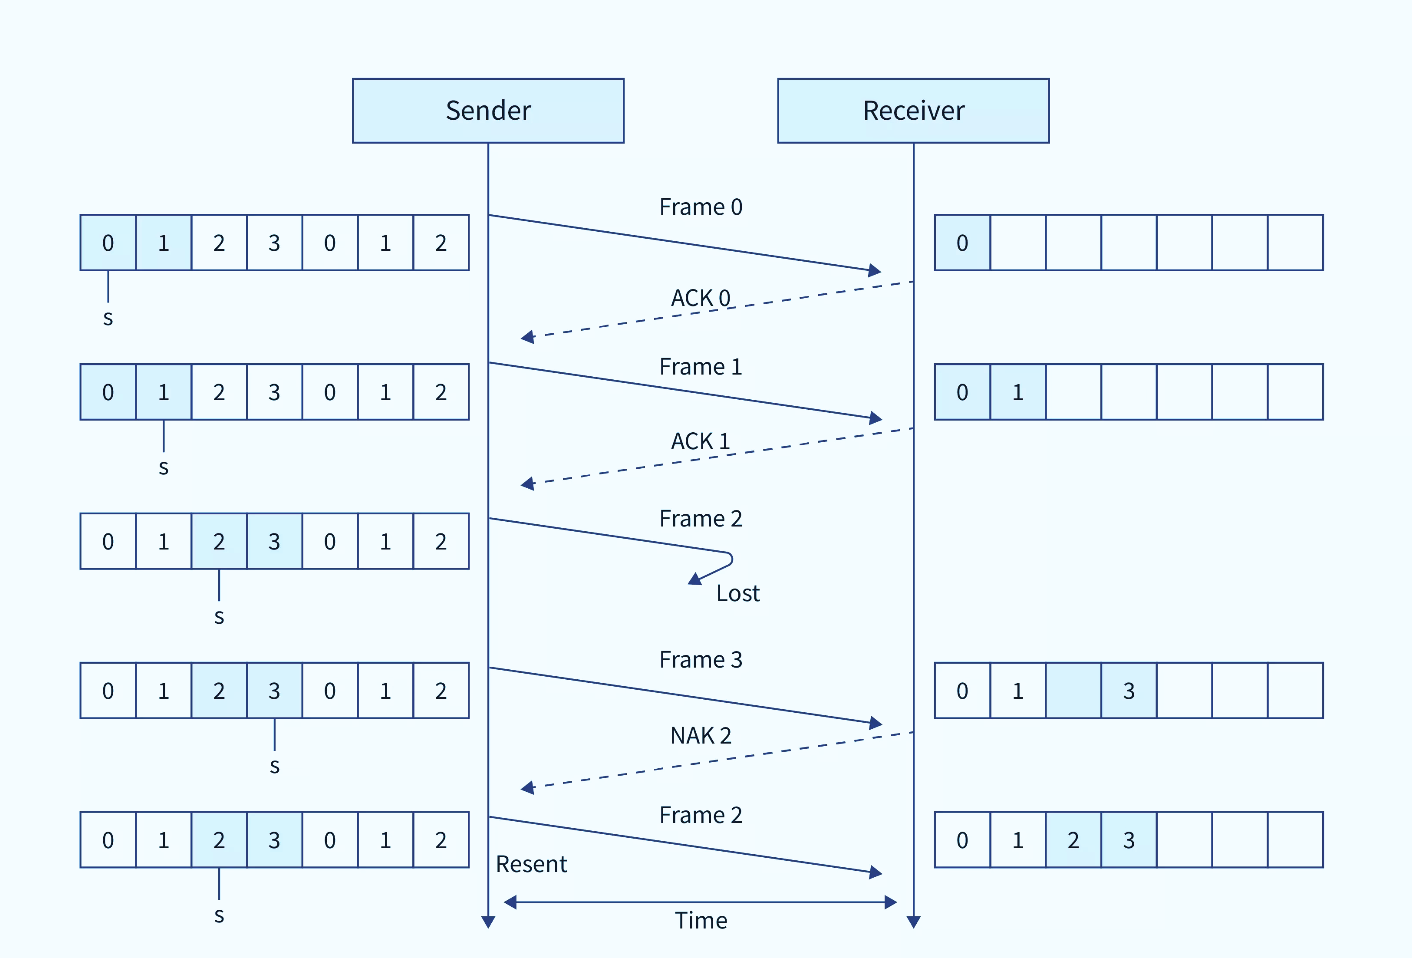
\includegraphics[width=0.75\textwidth]{imgs/01/sr.png}
    \caption{Funzionamento del protocollo \textit{Selective Repeat} \emoji{incoming-envelope}.}
\end{figure}

\section{Scelte progettuali}

\subsection{Gestione della concorrenza tramite processi \emoji{link}}
Il server è stato progettato come applicazione multi-processo in grado di gestire connessioni multiple.
Ogni volta che un nuovo client si connette, il server crea un processo figlio dedicato esclusivamente a quella connessione.
Questo approccio garantisce:
\begin{enumerate}
    \item \textbf{Isolamento dalle sessioni:} un malfunzionamento di un client non influisce sugli altri. Questo rende il sistema più robusto e resiliente ai guasti;
    \item \textbf{Semplicità gestionale:} evita complessità legate al multithreading, come race condition o deadlock.
\end{enumerate}

\subsection{Bitmask \emoji{red-square}\emoji{green-square}}
Per tenere traccia degli slot disponibili, affinché un generico client possa connettersi al server, quest'ultimo fa uso di una bitmask.
La bitmask è un array di bit, in cui ogni bit rappresenta lo stato di uno slot come mostrato in Fig. \ref{fig:bitmask}.

\begin{figure}[h]
    \centering
    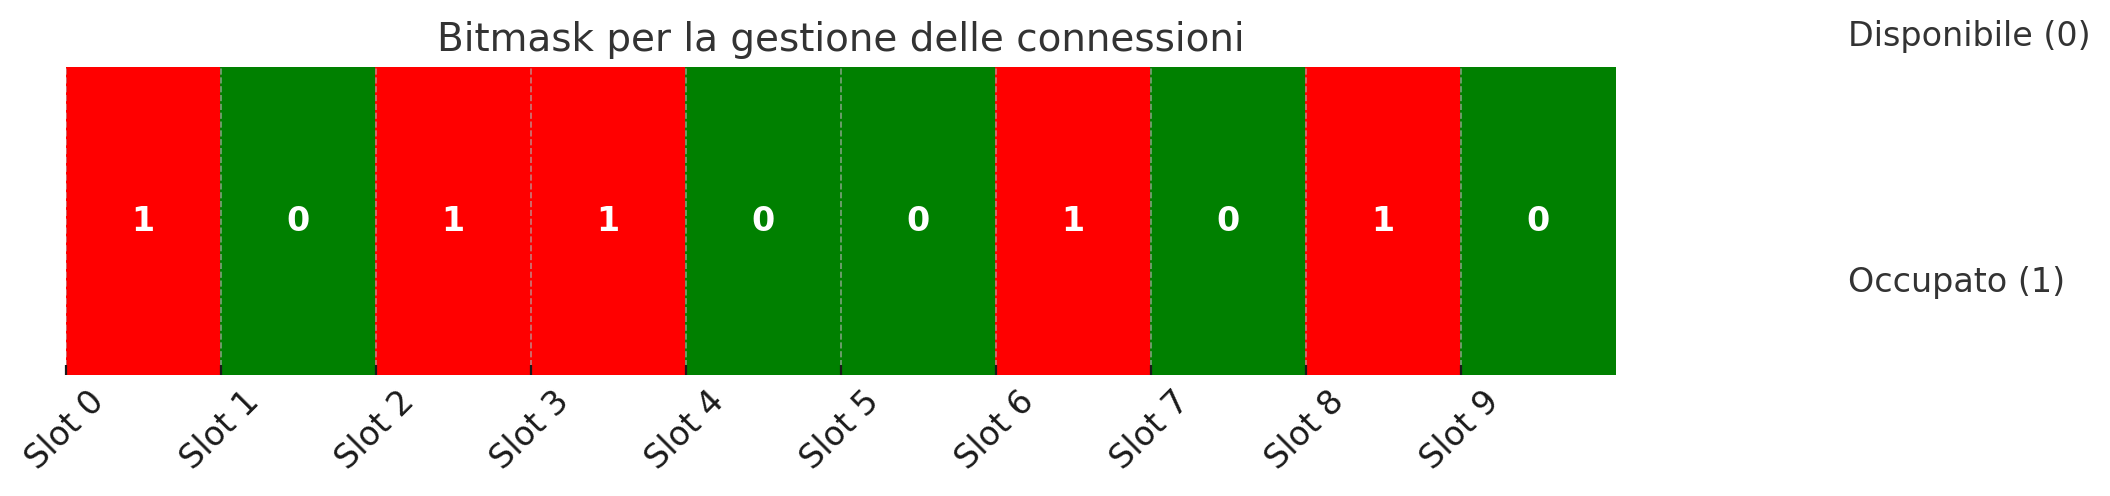
\includegraphics[width=0.75\textwidth]{imgs/01/bitmask.png}
    \caption{Rappresentazione grafica della bitmask.}
    \label{fig:bitmask}
\end{figure}

dove ogni bit della bitmask rappresenta un generico client connesso o meno al server.
Poichè si è scelto di poter accogliere al massimo $2727$ client, la bitmask è stata dimensionata per contenere $2727$ bit.
Questo implica che la dimensione della memoria condivisa, creata con le API di System V IPC, è di $341$ byte, calcolata come segue:

\begin{equation}
    \frac{2727}{8} = 341 \text{ byte} \nonumber
\end{equation}

\subsection{Casi particolari \emoji{police-car-light}}
Sia i client che il server sono dotati di handler per la gestione dei segnali, come \lstinlinebg{SIGINT} e \lstinlinebg{SIGQUIT}, garantendo una terminazione e una pulizia corretta delle risorse, sia nel caso in cui viene terminato prima il client, sia nel caso in cui viene terminato prima il server.
Inoltre è stato gestito il caso in cui il server è down e un generico client tenta di connettersi.
In questo caso il client termina l'esecuzione dopo tre tentativi di connessione falliti.
Per ultimo è stato gestito il caso in cui il server è occupato, ovvero tutti gli slot sono occupati, in questo caso il server notifica il client e quest'ultimo termina l'esecuzione.

\subsection{Timeout di inattività \emoji{three-oclock}}
L'applicazione prevede un meccanismo di timeout per la chiusura automatica delle connessioni inattive.
Si è considerato un tempo di inattività di 3600 secondi (1 ora) come limite massimo di tempo per la connessione.
Se un client non invia alcun messaggio al server per un periodo di tempo superiore a 1 ora, la connessione viene chiusa automaticamente dal server.
Questo meccanismo previene la persistenza di connessioni ``zombie" e garantisce un utilizzo efficiente delle risorse del server.

\subsection{Gestione degli errori e pacchetti persi \emoji{collision}\emoji{package}}
L'applicazione interrompe il trasferimento se si verificano più di $25$ errori consecutivi.
Questo numero è stato scelto per evitare che il protocollo di trasferimento dati entri in uno stato di loop infinito, ad esempio a causa della perdita o corruzione dei pacchetti.
Oltre questo limite, la quantità di dati corrotti renderebbe impossibile la ricostruzione fedele del file, compromettendone l'integrità e l'usabilità.

\subsection{Three-Way Handshake \emoji{handshake}}
Per stabilire una connessione tra client e server, è stato implementato un \textit{Three-Way Handshake} per garantire l'affidabilità e l'integrità della connessione.
Il \textit{Three-Way Handshake} è un protocollo di comunicazione a tre passaggi che consente a due host di stabilire una connessione TCP/IP.
Il protocollo funziona come segue:
\begin{enumerate}
    \item Il client invia un pacchetto di richiesta di connessione al server, contenente il flag \lstinlinebg{SYN} (synchronization request).
    \item Il server risponde con un pacchetto di conferma, contenente il flag \lstinlinebg{SYN} e \lstinlinebg{ACK} (acknowledgment).
    \item Il client invia un pacchetto di conferma al server, contenente il flag \lstinlinebg{ACK}.
    \item La connessione è stabilita e i due host possono iniziare a scambiarsi dati.
\end{enumerate}

\subsubsection{Three-Way Handshake di apertura}
Per la realizzazione del software S.P.Q.R. è stato implementato un \textit{Three-Way Handshake} di apertura per stabilire la connessione tra client e server.
Il client invia un pacchetto di richiesta di connessione al server, contenente il flag \lstinlinebg{SYN}.
Il server risponde con un pacchetto di conferma, contenente il flag \lstinlinebg{SYN-ACK}.
Infine, il client invia un pacchetto di conferma al server, contenente il flag \lstinlinebg{ACK}.
La connessione è stabilita e i due host possono iniziare a scambiarsi dati.

\begin{figure}[h]
    \centering
    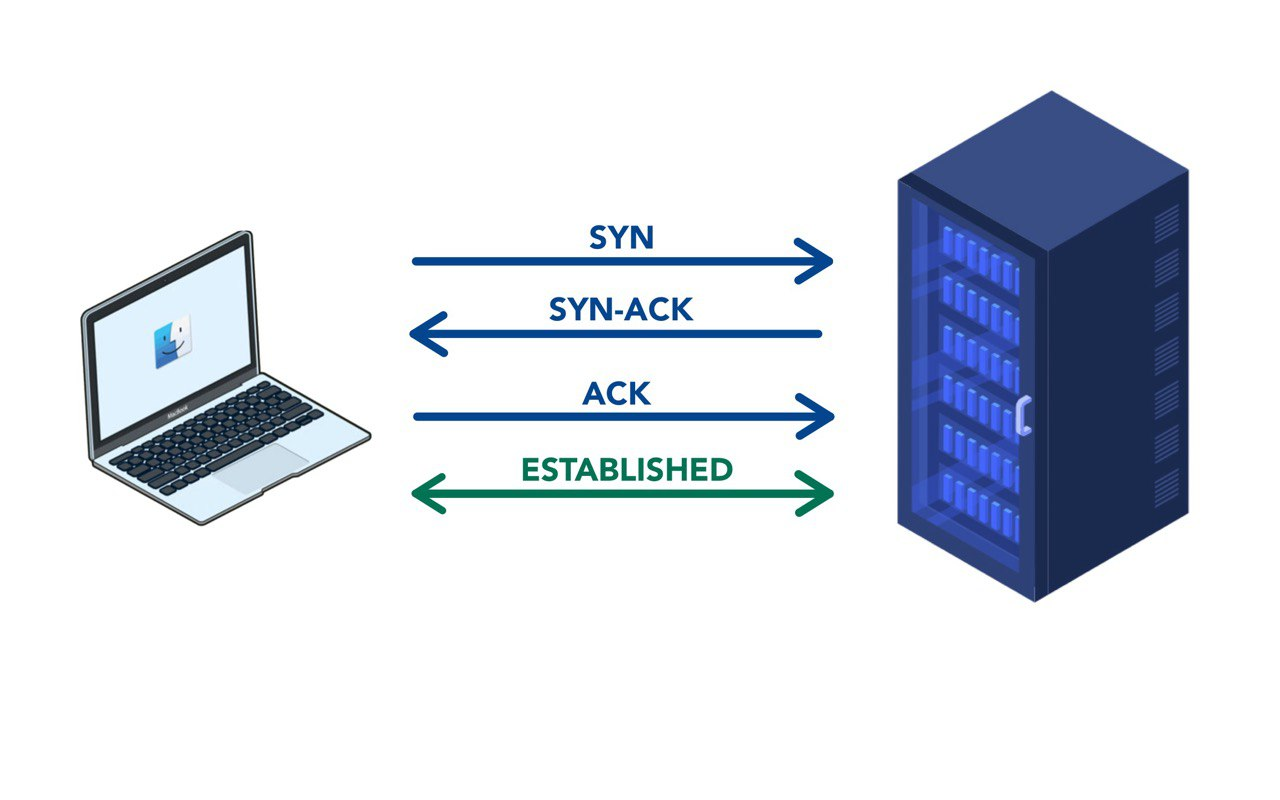
\includegraphics[width=0.65\textwidth]{imgs/02/macbook_server.jpeg}
    \caption{Three-Way Handshake d'apertura.}
\end{figure}

\subsubsection{Three-Way Handshake di chiusura}
Lo stesso vale per il \textit{Three-Way Handshake} di chiusura, che consente a client e server di terminare la connessione in modo sicuro.
Il client invia un pacchetto di richiesta di chiusura al server, contenente il flag \lstinlinebg{FIN}.
Il server risponde con un pacchetto di conferma, contenente il flag \lstinlinebg{FINACK} e invia un pacchetto di conferma al client, contenente il flag \lstinlinebg{FIN}.
Il client risponde con un pacchetto di conferma al server, contenente il flag \lstinlinebg{ACK}.
La connessione è chiusa e i due host possono liberare le risorse allocate.

\begin{figure}[h]
    \centering
    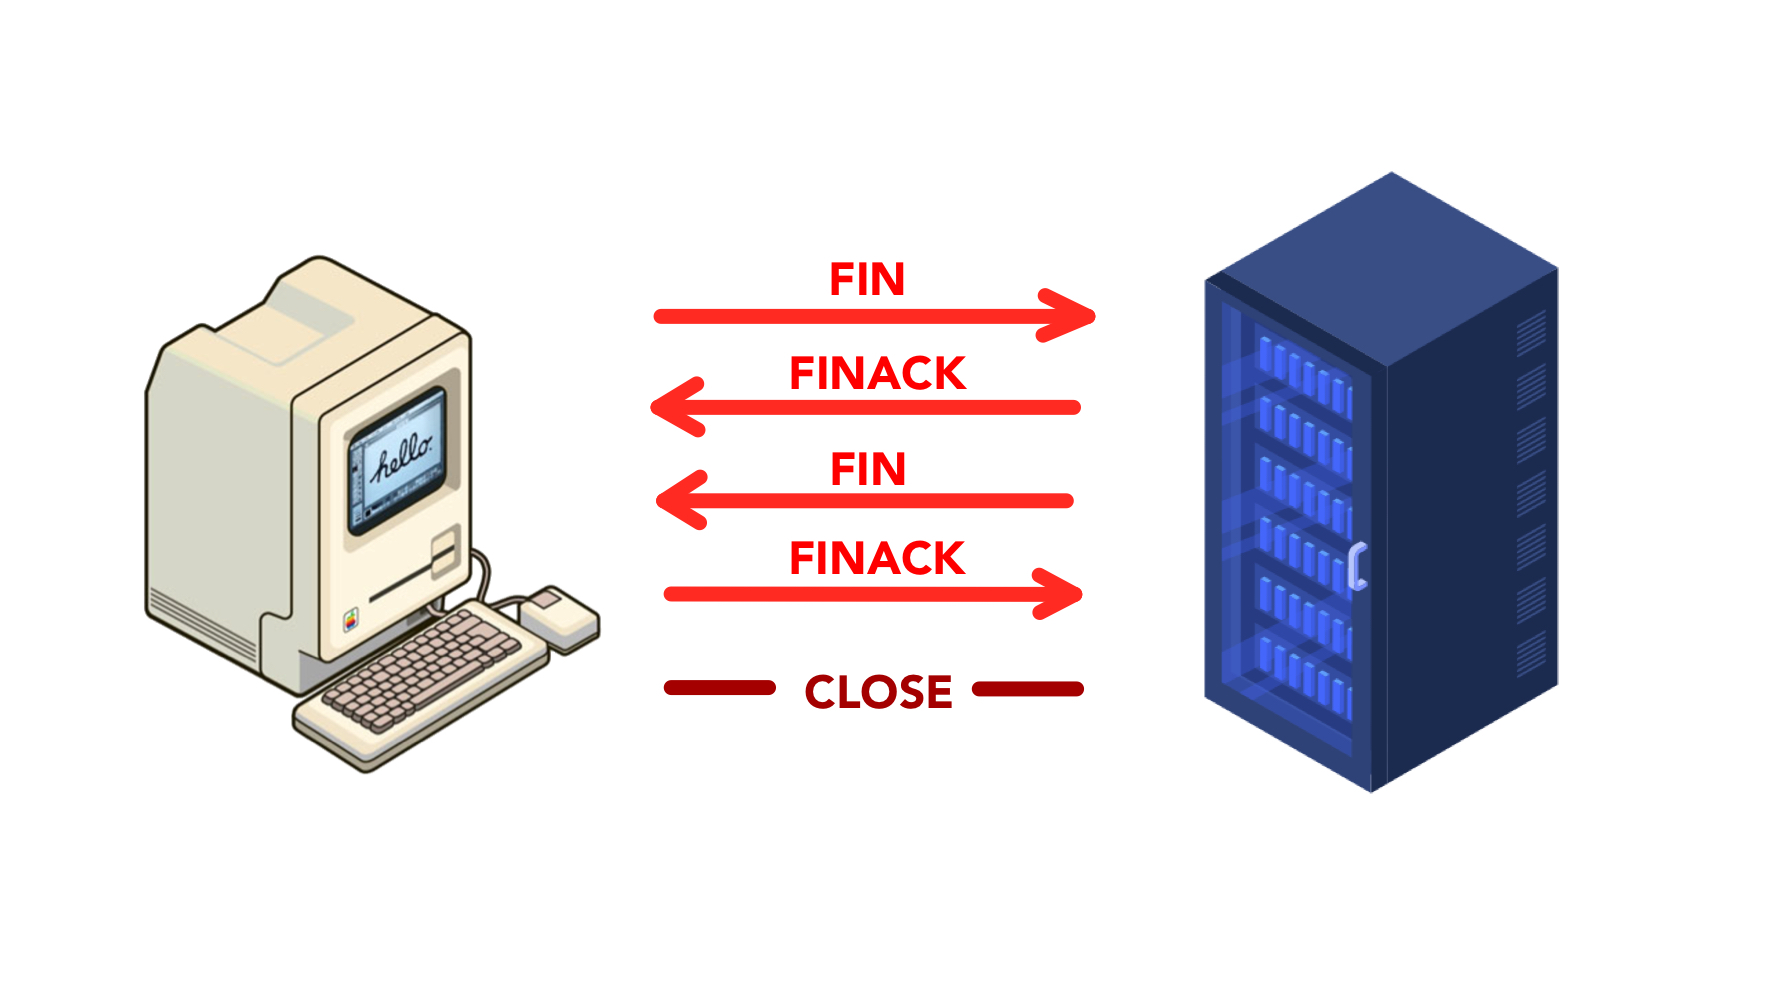
\includegraphics[width=0.65\textwidth]{imgs/02/three-way-handshake-chiusura.jpeg}
    \caption{Three-Way Handshake di chiusura.}
\end{figure}

\subsection{Progressive Bar \emoji{rocket}}
Per rendere il trasferimento dei file più interattivo e coinvolgente, è stata implementata una barra di avanzamento.
La barra di avanzamento mostra la percentuale di completamento del trasferimento, aggiornata in tempo reale.
Questo permette all'utente di monitorare il progresso del trasferimento e di avere un'idea chiara del tempo rimanente.

\begin{figure}[ht]
    \centering
    \animategraphics[autoplay,loop,width=0.95\textwidth]{100}{image/progressive-bar-}{0}{151}
    \caption{Animazione della progressive bar.}
\end{figure}
